\documentclass[a4paper,12pt]{article}
\usepackage[top = 2.5cm, bottom = 2.5cm, left = 2.5cm, right = 2.5cm]{geometry}
\usepackage[T1]{fontenc}
\usepackage[utf8]{inputenc}
\usepackage{multirow} 
\usepackage{booktabs} 
\usepackage{graphicx}
\usepackage[spanish]{babel}
\usepackage{setspace}
\setlength{\parindent}{0in}
\usepackage{float}
\usepackage{fancyhdr}
\usepackage{amsmath}
\usepackage{amssymb}
\usepackage{amsthm}
\usepackage[numbers]{natbib}
\newcommand\Mycite[1]{%
	\citeauthor{#1}~[\citeyear{#1}]}
\usepackage{graphicx}
\usepackage{subcaption}
\usepackage{booktabs}
\usepackage{etoolbox}
\usepackage{minibox}
\usepackage{hyperref}
\usepackage{xcolor}
\usepackage{pdfpages}
\usepackage[skins]{tcolorbox}
%---------------------------

\newtcolorbox{cajita}[1][]{
	 #1
}

\newenvironment{sol}
{\renewcommand\qedsymbol{$\square$}\begin{proof}[\textbf{Solución.}]}
	{\end{proof}}

\newenvironment{dem}
{\renewcommand\qedsymbol{$\blacksquare$}\begin{proof}[\textbf{Demostración.}]}
	{\end{proof}}

\newtheorem{problema}{Problema}
\newtheorem{definicion}{Definición}
\newtheorem{ejemplo}{Ejemplo}
\newtheorem{teorema}{Teorema}
\newtheorem{corolario}{Corolario}[teorema]
\newtheorem{lema}[teorema]{Lema}
\newtheorem{prop}{Proposición}
\newtheorem*{nota}{\textbf{NOTA}}
\renewcommand\qedsymbol{$\blacksquare$}
\usepackage{svg}
\usepackage{tikz}
\usepackage[framemethod=default]{mdframed}
\global\mdfdefinestyle{exampledefault}{%
linecolor=lightgray,linewidth=1pt,%
leftmargin=1cm,rightmargin=1cm,
}




\newenvironment{noter}[1]{%
\mdfsetup{%
frametitle={\tikz\node[fill=white,rectangle,inner sep=0pt,outer sep=0pt]{#1};},
frametitleaboveskip=-0.5\ht\strutbox,
frametitlealignment=\raggedright
}%
\begin{mdframed}[style=exampledefault]
}{\end{mdframed}}
\newcommand{\linea}{\noindent\rule{\textwidth}{3pt}}
\newcommand{\linita}{\noindent\rule{\textwidth}{1pt}}

\AtBeginEnvironment{align}{\setcounter{equation}{0}}
\pagestyle{fancy}

\fancyhf{}









%----------------------------------------------------------
\lhead{\footnotesize Data Science I}
\rhead{\footnotesize  Rudik Roberto Rompich}
\cfoot{\footnotesize \thepage}


%--------------------------

\begin{document}
 \thispagestyle{empty} 
    \begin{tabular}{p{15.5cm}}
    \begin{tabbing}
    \textbf{Universidad del Valle de Guatemala} \\
    Departamento de Ciencias de la Computación\\\\
   \textbf{Estudiantes:} Augusto Alonso, Angel Cuellar, Rudik Roberto Rompich\\
    \end{tabbing}
    \begin{center}
        CC3066 - Data Science I - Catedrático: Luis Furlan\\
        \today
    \end{center}\\
    \hline
    \\
    \end{tabular} 
    \vspace*{0.3cm} 
    \begin{center} 
    {\Large \bf  Proyecto 2 - Análisis Exploratorio 
} 
        \vspace{2mm}
    \end{center}
    \vspace{0.4cm}
%--------------------------

\textbf{Instrucciones:} El modelo que se desarrolló en clase tiene una precisión ya bastante alta.  Sin embargo, hay varios ajustes que se pueden intentar para mejorarlo. Es importante poner atención al tiempo que se tarda cada época en ejecutar. Utilizando el código visto en clase, experimenten con  los hiperparámetros del algoritmo.

\begin{figure}[H]
	\centering
	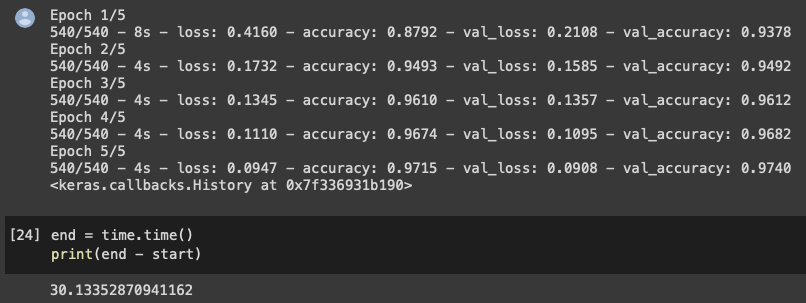
\includegraphics[scale=0.5]{Images/1.png}
	\caption{Caso base hecho en clase.}
\end{figure}
\section{Problemas}

\begin{problema}
	El ancho (tamaño de la capa escondida) del algoritmo. Intenten con un tamaño de 200.  
	\begin{figure}[H]
		\centering
		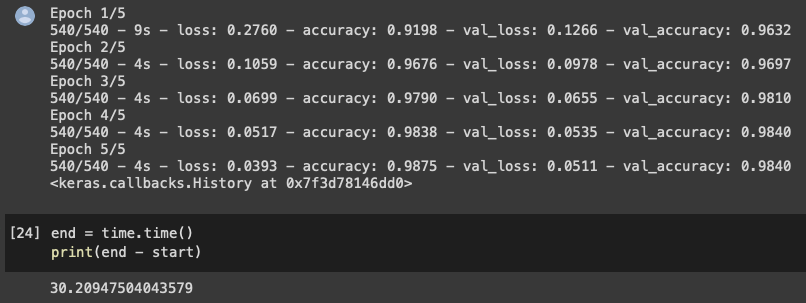
\includegraphics[scale=0.5]{Images/2.png}
		\caption{Tamaño de capa escondida de 200.}
	\end{figure}
	\begin{enumerate}
		\item ¿Cómo cambia la precisión de validación del modelo? 
			\begin{sol}
			Comparado al modelo original, en la quinta época se obtiene una mejora de 2\% en la precisión del modelo. 
		\end{sol}
		\item ¿Cuánto tiempo se tardó el algoritmo en entrenar?
			\begin{sol}
			30.209 segundos en entrenar; levemente más tardado que en el caso original. 
		\end{sol}
		\item ¿Puede encontrar un tamaño de capa escondida que funcione mejor?
			\begin{sol}
			Se compararon los siguientes casos: 
			\begin{table}[H]
				\centering
				\label{tab:comparacion}
				\begin{tabular}{@{}cccc@{}}
					\toprule
					\textbf{Tamaño capa} & \textbf{Épocas} & \textbf{Tiempo (s)} & \textbf{Precisión} \\ \midrule
					50                   & 5               & 30.13               & 97.4\%             \\
					200                  & 5               & 30.20               & 98.4\%             \\
					300                  & 5               & 42.14               & 98.65\%            \\
					400                  & 5               & 50.94               & 98.33\%            \\ \bottomrule
				\end{tabular}
			\caption{Tamaños de capa}
			\end{table}
		En conclusión, a partir de la capa 200 ya se cuenta con una precisión excelente y agregar capas no necesariamente mejorar el modelo, como sucede en la el tamaño de capa de 400 que presenta un porcentaje más bajo que en el tamaño de capa de 300. Por lo que se recomendaría usar un tamaño de capa levemente superior a 200. 
		\end{sol}
	\end{enumerate}
\end{problema}


%---------------

\begin{problema}
	La profundidad del algoritmo.  Agreguen una capa escondida más al algoritmo. ¡Este es un ejercicio extremadamente importante! 
	\begin{figure}[H]
		\centering
		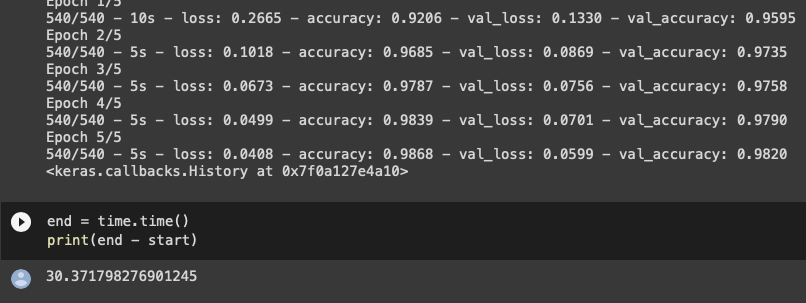
\includegraphics[scale=0.5]{Images/3.png}
		\caption{Capa extra.}
	\end{figure}
	\begin{enumerate}
		\item  ¿Cómo cambia la precisión de validación?  
		\begin{sol}
			Comparado al caso anterior, hubo una disminución del 0.2\% en la precisión del algoritmo.  
		\end{sol}
		\item ¿Qué hay del tiempo que se tarda en ejecutar?   Pista:  deben tener cuidado con las formas de los pesos y los sesgos.
		\begin{sol}
			El tiempo es prácticamente el mismo; un poco mayor por centésimas de segundo. 
		\end{sol}
	\end{enumerate}
\end{problema}
%---------------
\begin{problema}
	El ancho y la profundidad del algoritmo.  Agregue cuantas capas sean necesarias para llegar a 5 capas escondidas.  Es más, ajusten el ancho del algoritmo conforme lo encuentre más conveniente. 
		\begin{figure}[H]
		\centering
		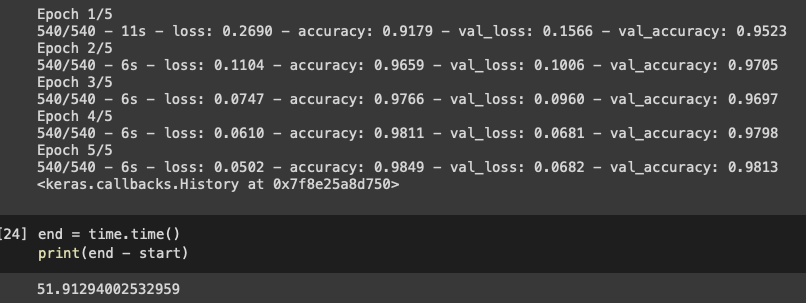
\includegraphics[scale=0.5]{Images/4.png}
		\caption{5 capas.}
	\end{figure}
	\begin{enumerate}
		\item ¿Cómo cambia la precisión de validación? 
		\begin{sol}
			Es levemente peor al caso anterior; lo que quiere decir que agregar capas no hace al modelo más efectivo. 
		\end{sol}
		\item ¿Qué hay del tiempo de ejecución?
		\begin{sol}
			Llega a casi 52 segundos; por lo cual no es tan eficiente comparado a los casos anteriores. 
		\end{sol}
	\end{enumerate} 
\end{problema}
%---------------
\begin{problema}
	Experimenten con las funciones de activación.  Intenten aplicar una transformación sigmoidal a ambas capas.  La activación sigmoidal se obtiene escribiendo “sigmoid”.
	\begin{sol} Los resultados aparentan ser levemente peores y el tiempo no tiene ningún cambio. 
		\begin{figure}[H]
			\centering
			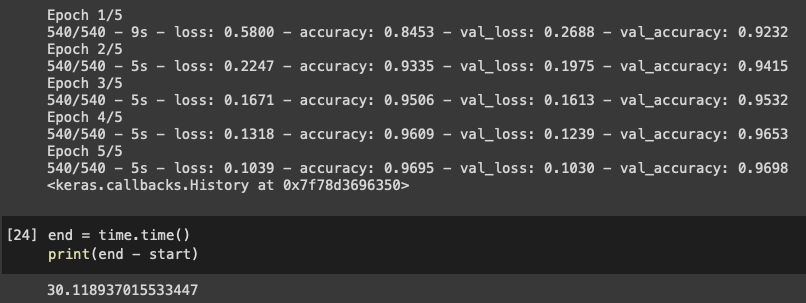
\includegraphics[scale=0.5]{Images/5.png}
			\caption{Función «sigmoid».}
		\end{figure}
	\end{sol}
\end{problema}
%---------------
\begin{problema}
	Continúen experimentando con las funciones de activación.  Intenten aplicar un ReLu a la primera capa escondida y $\tanh$ a la segunda.  La activación tanh se obtiene escribiendo “tanh”.
		\begin{figure}[H]
		\centering
		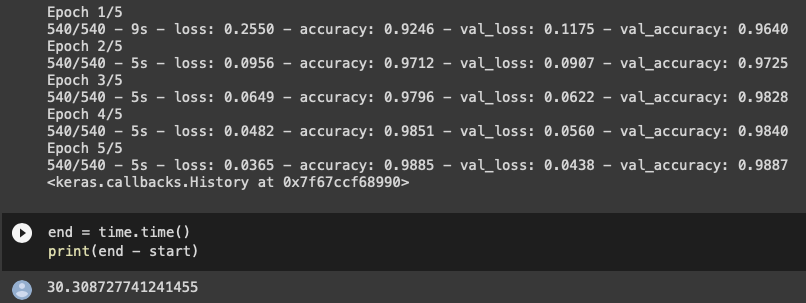
\includegraphics[scale=0.5]{Images/6.png}
		\caption{Activación ReLu y tanh.}
	\end{figure}
	\begin{sol}
	 En cuestiones de eficiencia; el tiempo es similar a los demás casos. Por otra parte, la precisión de la validación es la más alta de todos los casos con 98.87\% de precisión. 
	\end{sol}
\end{problema}
%---------------
\begin{problema}
	Ajusten el tamaño de la tanda.  Prueben con un tamaño de tanda de 10,000.  
		\begin{figure}[H]
		\centering
		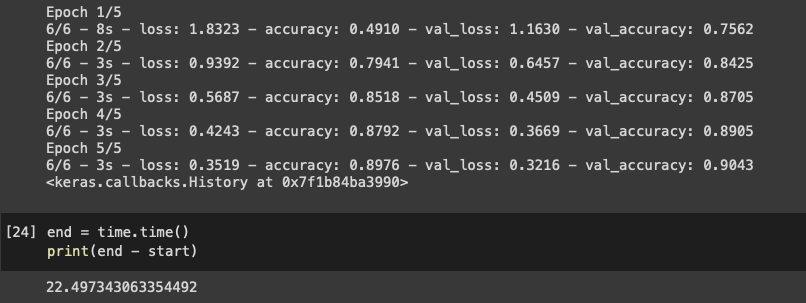
\includegraphics[scale=0.5]{Images/7.png}
		\caption{Tamaño de tanda de 10,000.}
	\end{figure}
	
	\begin{enumerate}
		\item ¿Cómo cambia el tiempo requerido?
		\begin{sol}
			El tiempo es de 22.50 segundos, siendo el caso más eficiente. 
		\end{sol}
		\item ¿Cómo cambia la precisión?
		\begin{sol}
			La precisión es la más baja hasta ahora; con un 90\% de precisión.		\end{sol}
	\end{enumerate}
\end{problema}
%---------------
\begin{problema}
	Ajusten el tamaño de la tanda a 1.  Eso corresponde al SGD.
	\begin{figure}[H]
		\centering
		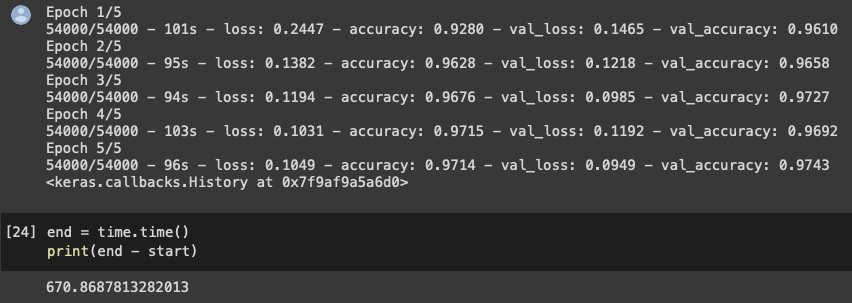
\includegraphics[scale=0.5]{Images/8.png}
		\caption{Tamaño de la tanda 1.}
	\end{figure}
	\begin{enumerate}
		\item  ¿Cómo cambian el tiempo y la precisión? 
		\begin{sol}
			El tiempo se dispara drásticamente (671 segundos); aunque la precisión es bastante normal, alrededor de 97\%. 
		\end{sol}
		\item  ¿Es el resultado coherente con la teoría?
		\begin{sol}
			En efecto, la teoría se cumple; ya que el descenso del gradiente está al principio y por eso se tarda un largo rato en cargar el modelo. 
		\end{sol}
	\end{enumerate}
	
\end{problema}
%---------------
\begin{problema}
	Ajusten la tasa de aprendizaje.  Prueben con un valor de 0.0001.  ¿Hace alguna diferencia?
	\begin{figure}[H]
		\centering
		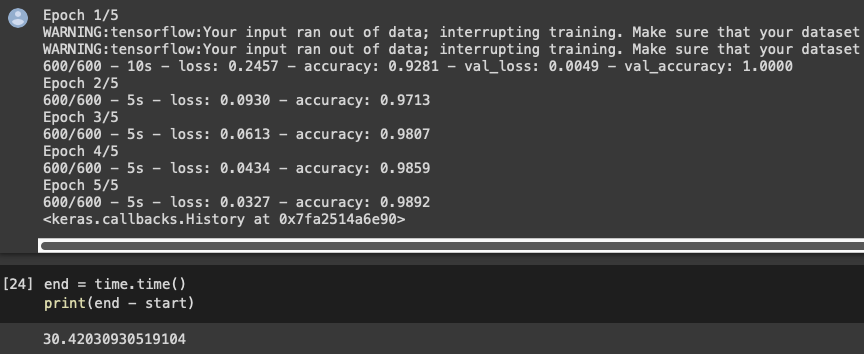
\includegraphics[scale=0.5]{Images/9.png}
		\caption{Valor de 0.0001.}
	\end{figure}
	\begin{sol}
		El tiempo es básicamente promedio; mientras que la precisión llega a 98.92\% de precisión; aunque la librería lanza un error respecto  a posibles datos erróneos.  
	\end{sol}
\end{problema}
%---------------
\begin{problema}
	Ajusten la tasa de aprendizaje a 0.02.  ¿Hay alguna diferencia?
		\begin{figure}[H]
		\centering
		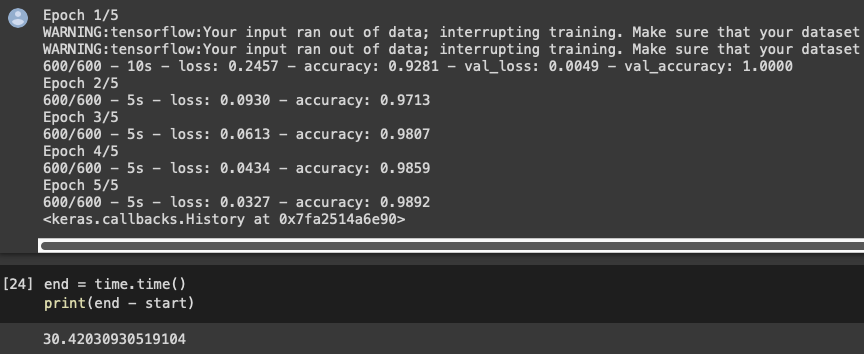
\includegraphics[scale=0.5]{Images/9.png}
		\caption{Valor de 0.02.}
	\end{figure}
	\begin{sol}
		Hasta el momento, esta elección representa el modelo más preciso con 99.33\% y 30.42 segundos. 
	\end{sol}
\end{problema}
%---------------
\begin{problema}
	Combinen todos los métodos indicados arriba e intenten llegar a una precisión de validación de 98.5\% o más.
	\begin{sol}
		Las siguientes opciones son las mejores para obtener una precisión de 99.33\%:
	\begin{enumerate}
		\item Dos capas: 
		\begin{enumerate}
			\item Primera capa con inicialización ReLu. 
			\item Segunda capa con inicialización tanh. 
		\end{enumerate}
	\item Tasa de aprendizaje de 0.02. 
	\item Tamaña de tanda: 100. 
	\item Tamaño de capa escondida: 200. 
\end{enumerate}	\end{sol}
\end{problema}
%---------------





%---------------------------
\bibliographystyle{apa}
\bibliography{referencias.bib}

\end{document}